
\begin{frame}{Các thách thức với RAN}
  Khi số lượng thuê bao và ứng dụng di động bùng nổ, MNO phải tối ưu tất cả thành phần mạng, trong đó RAN thường chiếm phần lớn chi phí triển khai và vận hành.

    \vspace{0.2cm}

  Sự ra đời của 5G đưa đến 3 use cases mới:
  \begin{itemize}
    \item Enhanced Mobile Broadband (\textbf{eMBB}): Ưu tiên băng thông cao cho streaming, download/upload lớn.
    \item Ultra-Reliable Low-Latency Communication (\textbf{URLLC}): Ưu tiên độ trễ siêu thấp và độ tin cậy cực cao cho các ứng dụng như điều khiển robot, phẫu thuật từ xa.
    \item Massive Machine-Type Communication (\textbf{mMTC}): Ưu tiên kết nối số lượng thiết bị cực lớn với lưu lượng mỗi thiết bị rất nhỏ (IoT, sensor).
  \end{itemize}

  \vspace{0.2cm}
  Mọi ứng dụng và mọi thiết bị không dây đều có các yêu cầu QoS riêng. RAN nguyên khối hiện tại không thể đáp ứng các yêu cầu đa dạng của các trường hợp sử dụng này.Khi cố gắng đưa cả eMBB, URLLC và mMTC vào chung một “đường ống” RAN, sẽ phải hy sinh 1 trong 3 yêu cầu dấn đến giảm sút QoS và QoE.     

\end{frame}

\begin{frame}{Các thách thức với RAN}
  Một thách thức khác đối với RAN là kết hợp NFV hiện có với trí tuệ nhân tạo (AI). Xu hướng NFV đã tồn tại kể từ khi phát triển từ C-RAN lên vRAN.
  \begin{block}{NFV}
    NFV (Network Function Virtualization) đã cho phép ảo hóa các chức năng mạng (như BBU, DU, CU) thành các ứng dụng phần mềm chạy trên phần cứng chung.
  \end{block}
  Cần một cơ chế quản lý và điều phối, may mắn thay việc này có thể được thực hiện bằng cách tận dụng AI. AI có thể được sử dụng để phân tích lượng dữ liệu khổng lồ do RAN tạo ra. Sau đó, thông tin thu thập được có thể được sử dụng để dự đoán các sự cố trong mạng và thực hiện hành động cần thiết để đảm bảo QoS mạng được cung cấp cho người dùng. AI có thể làm cho hệ thống NFV thông minh hơn, được tối ưu hóa và cải thiện hơn. 
  
\end{frame}

\begin{frame}{Các thách thức với RAN}
  \begin{columns}[T]
    % ——————— Cột chữ ———————
    \column{0.6\textwidth}
    Phần mềm nhúng AI là cần thiết để hoàn thành quá trình phát triển NFV. Chính việc này lại đặt ra vấn đề là các MNO không thể triển khai NFV nhúng AI vì họ phụ thuộc vào việc các nhà cung cấp đối tác của họ có cung cấp giải pháp này hay không.phần mềm và phần cứng của RAN là độc quyền và chỉ được tối ưu hóa cho một nhà cung cấp. Điều này gây ra tình trạng độc quyền kinh tế với chi phí cực kỳ cao và dẫn đến các hệ thống không được giám sát vì nhà cung cấp duy nhất có thể cung cấp phần cứng và phần mềm là nhà cung cấp đó.

    % ——————— Cột hình ———————
    \column{0.4\textwidth}
    \centering
    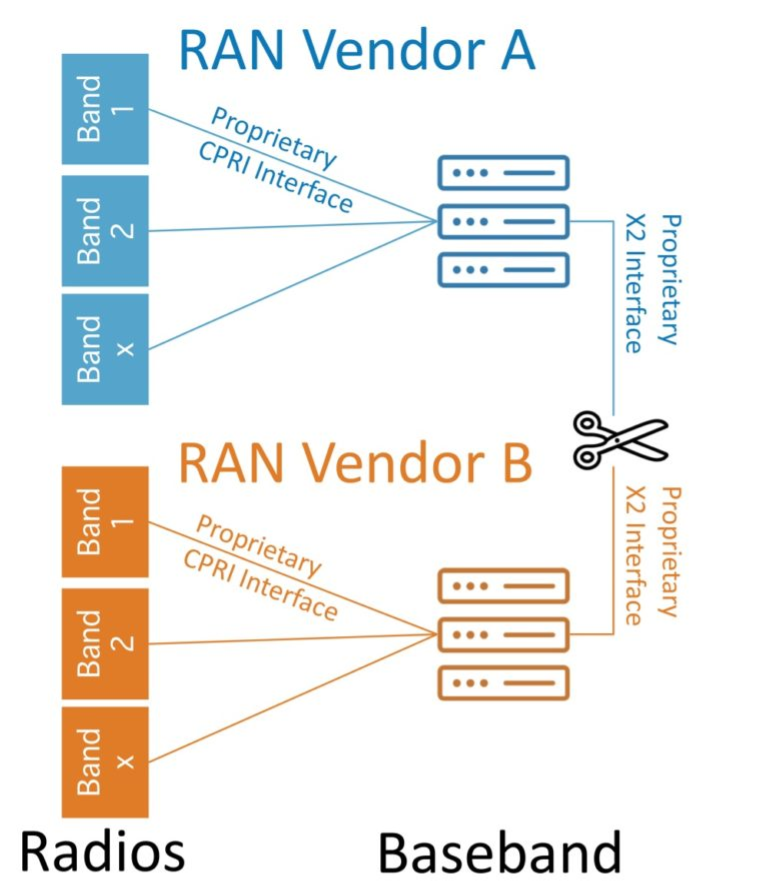
\includegraphics[height=6cm, keepaspectratio]{picture/vendor_simu.png}
    \\[1ex]
  \end{columns}
\end{frame}

\begin{frame}{Open RAN}
  \begin{columns}[T]
    % ——————— Cột chữ ———————
    \column{0.6\textwidth}
    \vspace{0.4cm}
    Open RAN là một kiến trúc RAN mới, được xây dựng dựa trên nguyên tắc: \textbf{phân tách (disaggregation)} và \textbf{tương tác (interoperability)}:

    \begin{itemize}
      \item \textbf{Disaggregation}: Phần mềm mạng được tách rời khỏi phần cứng.
      \item \textbf{Interoperability}: Các thành phần từ nhiều nhà cung cấp có thể hoạt động cùng nhau.
    \end{itemize}

    Khác với các thế hệ RAN trước vốn sử dụng hệ thống độc quyền một nhà cung cấp, Open RAN sử dụng giao diện mở và phần mềm độc lập với phần cứng, có thể triển khai trên bộ xử lý phổ thông.

    % ——————— Cột hình ———————
    \column{0.4\textwidth}
    \centering
    \vspace{0.5cm}
    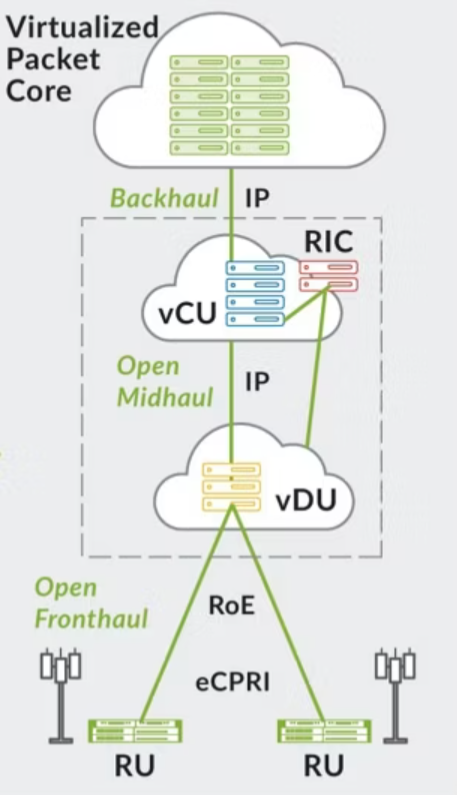
\includegraphics[height=6cm, keepaspectratio]{picture/oRan.png}
    \\[1ex]
  \end{columns}
\end{frame}

\begin{frame}{Lợi ích và đột phá của Open RAN}
  Open RAN mang lại nhiều lợi ích thiết thực cho nhà mạng:
  \begin{itemize}
    \item Cho phép triển khai kiến trúc đa nhà cung cấp.
    \item Giảm chi phí đầu tư và chi phí vận hành
    \item Tăng tốc độ triển khai dịch vụ với mô hình CI/CD.
    \item Tích hợp AI/ML để tự động hóa, phát hiện và xử lý sự cố.
    \item Cải thiện khả năng mở rộng và thích ứng QoS.
  \end{itemize}

  \vspace{0.3cm}
  Ví dụ thực tiễn -- \textbf{Rakuten Mobile (Nhật Bản)}:
  \begin{itemize}
    \item Mạng thương mại toàn quốc đầu tiên triển khai Open RAN.
    \item Đạt điểm hiệu suất \textbf{920/1000} theo đánh giá Umlaut.
    \item Tiết kiệm tới \textbf{50\% chi phí} khi triển khai mạng 5G so với RAN truyền thống.
  \end{itemize}
\end{frame}
